\documentclass[11pt,a4paper]{article}

\usepackage[utf8]{inputenc}
\usepackage[T1]{fontenc}
\usepackage{lmodern}
\usepackage[margin=1in]{geometry}
\usepackage{hyperref}
\usepackage{booktabs}
\usepackage{listings}
\usepackage{xcolor}
\usepackage{amsmath}
\usepackage{graphicx}
\usepackage{natbib}
\usepackage{microtype}
\usepackage{tikz}

\definecolor{codebg}{rgb}{0.96,0.96,0.96}
\definecolor{keyword}{rgb}{0.5,0.0,0.5}
\definecolor{string}{rgb}{0.6,0.4,0.0}
\definecolor{comment}{rgb}{0.4,0.4,0.4}

\lstset{
  backgroundcolor=\color{codebg},
  basicstyle=\ttfamily\small,
  keywordstyle=\color{keyword}\bfseries,
  stringstyle=\color{string},
  commentstyle=\color{comment}\itshape,
  breaklines=true,
  frame=single,
  framerule=0pt,
  xleftmargin=1em,
  xrightmargin=1em,
  aboveskip=1em,
  belowskip=1em,
  numbers=left,
  numberstyle=\tiny\color{comment},
  numbersep=8pt,
}

\title{Parallel String Theory: Replacing Hierarchical Data Structures\\with Positional Identity and Constraint Solving}

\author{
  S.\ Seto\\
  \texttt{sseto001@gmail.com}\\
  \url{https://github.com/outconceive/pst-os}
}

\date{\today}

\begin{document}

\maketitle

% ===================================================================
\begin{abstract}
We present Parallel String Theory, a systems architecture that replaces hierarchical data structures with flat parallel strings and constraint-based relationships. Traditional operating systems manage processes, filesystems, scheduling, and IPC through trees and pointer graphs---structures that require pointer chasing, rebalancing, and cascading updates. We demonstrate that a single primitive---a flat table of parallel strings where identity is position, mutation is append-only, and relationships are declared as constraints solved by topological sort---is sufficient to implement all major OS subsystems. PST~OS, a 217KB operating system built on the formally verified seL4 microkernel, proves this claim empirically: it boots to a windowed desktop with keyboard input, persistence, networking, and a live Markout shell, without a single tree or pointer graph in its architecture. The same primitive independently validates in Outconceive~UI, a production web framework that replaces virtual DOM trees with parallel strings, proving the model generalizes across kernel space and userspace. We further introduce Markout, a declarative constraint-based UI language whose parametric layout solver extends the same topological sort from time (scheduling) to space (layout), unifying OS resource management and UI rendering under one abstraction.
\end{abstract}

% ===================================================================
\section{Introduction}

Every modern operating system organizes resources through hierarchical data structures. Process trees manage parent-child relationships. Directory trees locate files. Page tables map virtual to physical addresses. Priority queues order scheduling decisions. These structures work---they have worked for fifty years---but they carry inherent costs: pointer indirection, rebalancing on mutation, and cascading structural changes when a node is inserted or removed.

We ask: are trees \emph{necessary}, or are they merely the first solution that calcified into convention?

This paper presents an alternative. In our model, every resource---a process, a file, an IPC message, a scheduled task, a UI component---is a row in a flat table of parallel strings. Identity is not a pointer or a generated key; it is a position. Mutation is not an in-place update; it is an append. Deletion is not a structural removal; it is a tombstone marker, lazily compacted. Relationships between entities are not encoded in tree edges; they are declared as constraints and resolved by a topological sort.

We call this \emph{Parallel String Theory} (PST).

The contribution of this paper is threefold:

\begin{enumerate}
  \item A formal description of the parallel strings primitive and its invariants (Section~\ref{sec:primitive}).
  \item An empirical demonstration that this primitive is sufficient for all major OS subsystems: process management, filesystems, IPC, scheduling, and memory allocation (Section~\ref{sec:subsystems}).
  \item A proof that the same primitive generalizes beyond the kernel to UI rendering, unifying temporal constraint solving (scheduling) and spatial constraint solving (layout) under one algorithm (Section~\ref{sec:markout}).
\end{enumerate}

PST~OS is a working operating system---not a simulation---that boots on the formally verified seL4 microkernel~\citep{sel4} to a windowed desktop with keyboard input, disk persistence, TCP/IP networking, a text editor, a code stepper, and a Markout document browser, all in 217KB of statically linked Rust with no standard library.

% ===================================================================
\section{The Parallel Strings Primitive}
\label{sec:primitive}

\subsection{Definition}

A \texttt{ParallelTable} is an ordered sequence of rows, where each row is a fixed set of equal-length strings (columns). The canonical form uses four columns:

\begin{figure}[h]
\centering
\begin{lstlisting}[numbers=none]
content:    "Username  ________  Login "
components: "LLLLLLLLLLIIIIIIIIIIBBBBBB"
state_keys: "__________username__submit"
styles:     "                    pppppp"
\end{lstlisting}
\caption{A UI row as four parallel strings. A component is a contiguous column slice across all four strings. The label (L), input (I), and button (B) share no structural relationship---only positional adjacency.}
\label{fig:parallel}
\end{figure}

A \emph{component} is not a struct, a class, or a node---it is a contiguous column slice across all four strings. Its identity is its character offset. This identity never changes, even across compaction, because an \texttt{OffsetTable} maintains a mapping from logical positions to physical positions.

\subsection{Complexity comparison}

Table~\ref{tab:complexity} compares the asymptotic cost of core operations under tree-based and parallel-string-based architectures.

\begin{table}[h]
\centering
\begin{tabular}{lll}
\toprule
\textbf{Operation} & \textbf{Tree (traditional)} & \textbf{Parallel strings (PST)} \\
\midrule
Insert         & $O(\log n)$ + rebalance    & $O(1)$ append \\
Lookup by ID   & $O(\log n)$                & $O(1)$ offset table \\
Delete         & $O(\log n)$ + cascade      & $O(1)$ tombstone \\
Range query    & $O(\log n + k)$            & $O(n)$ prefix scan \\
Compaction     & N/A                        & $O(n)$ with offset remap \\
\bottomrule
\end{tabular}
\caption{Asymptotic complexity of core operations. Parallel strings trade $O(\log n)$ range queries for $O(1)$ insert, lookup, and delete. Compaction is deferred and amortized.}
\label{tab:complexity}
\end{table}

The tradeoff is explicit: $O(1)$ mutation and lookup in exchange for $O(n)$ scans. For OS resource tables (hundreds to thousands of entries), the scan cost is negligible. Section~\ref{sec:limitations} discusses scaling behavior.

\subsection{Invariants}

The primitive enforces five invariants:

\begin{enumerate}
  \item \textbf{Positional identity.} An entity's identity is its row index (and, within a row, its column offset). Identities are never reused.
  \item \textbf{Append-only mutation.} New entities are created by appending rows. No row is overwritten in place.
  \item \textbf{Tombstone deletion.} Removing an entity writes a tombstone marker at its position. The row remains until compaction.
  \item \textbf{Lazy compaction.} A compaction pass removes tombstoned rows and updates the offset table. Compaction is an $O(n)$ scan, not a tree rebalance.
  \item \textbf{Two immortal positions.} The system has exactly two positions that are never tombstoned and never compacted: the bootloader entry point and the offset table root.
\end{enumerate}

\subsection{Constraint relationships}

Entities declare relationships as constraints rather than encoding them structurally:

\begin{lstlisting}[language={},numbers=none]
Constraint::After("cryptod")      // temporal
Constraint::CenterX("title")      // spatial
Constraint::GapY(16, Some("header"))
\end{lstlisting}

A topological sort~\citep{toposort} over the constraint graph computes an execution order. Cycles in the constraint graph correspond to deadlocks; a watchdog process detects and tombstones them, and the solver resumes on the next tick.

This is the key architectural claim: \emph{constraint solving replaces hierarchy}. A process does not ``belong to'' a parent process via a tree edge. It declares ``I run after cryptod'' as a constraint, and the solver computes the ordering.

% ===================================================================
\section{OS Subsystems on Parallel Strings}
\label{sec:subsystems}

We implement six subsystems, each as a \texttt{ParallelTable} with domain-specific columns.

\subsection{Process table (\texttt{proctable})}

Each process is a row with columns: name, state, privilege level, priority, affinity, and a list of constraints. Boot order is computed by \texttt{solve\_spawn\_order()}, which runs the topological sort over \texttt{After} constraints.

\begin{lstlisting}
pt.register("vfs", PRIV_SYSTEM, vec![
    Constraint::After("cryptod".into()),
]);
let order = pt.solve_spawn_order();
// cryptod -> vfs -> netd -> compositor
\end{lstlisting}

Adding a new service with new constraints automatically adjusts the boot order. No hardcoded sequence, no init scripts.

\subsection{Filesystem (\texttt{pst-vfs})}

Files are rows. Directories are naming conventions. \texttt{ls} is a prefix scan over the name column. \texttt{find} is a substring search (grep). Delete is a tombstone. There is no directory tree to traverse.

\begin{lstlisting}
fs.ls("/home/");   // prefix scan -> [readme.md, notes.txt]
fs.find("readme"); // grep -> [/home/readme.md]
fs.delete(id);     // tombstone, not unlink
\end{lstlisting}

\subsection{IPC event log (\texttt{pst-ipc})}

Messages are append-only rows with sender, receiver, channel, priority, and payload columns. Delivery order is a priority-sorted scan over pending messages. Hardware interrupts are not a special mechanism---they are high-priority appends to the same log.

\subsection{Scheduler (\texttt{pst-sched})}

The scheduler is the constraint solver itself. Process constraints form a dependency graph; the topological sort produces an execution order. Blocked processes are rows whose constraints reference pending IPC messages. When a message arrives, the constraint is satisfied and the process re-enters the sorted order.

\subsection{Memory allocator (\texttt{pst-mem})}

Memory regions are rows with start address, length, owner, and status columns. Allocation appends a row. Deallocation tombstones it. Coalescing adjacent free regions is a scan over consecutive rows---the same operation as compaction.

\subsection{Temporal dimension (\texttt{pst-time})}

Time is a parallel string: each tick is a row with timestamp, delta, and retention policy columns. History is append-only by definition. Tiered compaction (fine-grained recent history, coarse-grained older history) is the same tombstone-and-compact operation applied temporally.

% ===================================================================
\section{Markout: Unifying Temporal and Spatial Constraints}
\label{sec:markout}

The constraint solver does not know or care whether it is solving for \emph{time} (``process A runs after process B'') or \emph{space} (``button X is centered below input Y''). Both are directed acyclic graphs resolved by the same topological sort.

\begin{figure}[h]
\centering
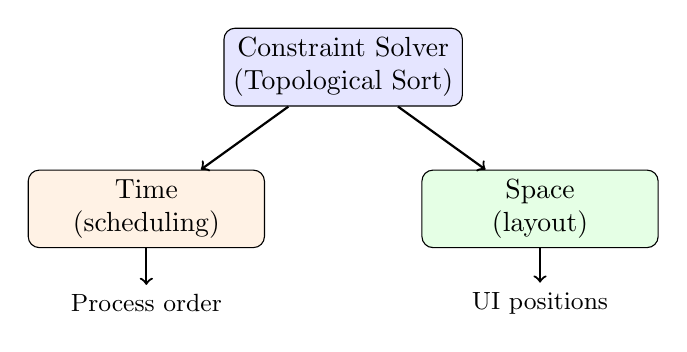
\begin{tikzpicture}[
  box/.style={draw, rounded corners, minimum width=3cm, minimum height=0.8cm, align=center},
  arrow/.style={->, thick},
]
  \node[box, fill=blue!10] (solver) at (0,3) {Constraint Solver\\(Topological Sort)};
  \node[box, fill=orange!10] (time) at (-2.5,1.2) {Time\\(scheduling)};
  \node[box, fill=green!10] (space) at (2.5,1.2) {Space\\(layout)};
  \node[align=center] (proc) at (-2.5,0) {\small Process order};
  \node[align=center] (ui) at (2.5,0) {\small UI positions};

  \draw[arrow] (solver) -- (time);
  \draw[arrow] (solver) -- (space);
  \draw[arrow] (time) -- (proc);
  \draw[arrow] (space) -- (ui);
\end{tikzpicture}
\caption{The constraint solver is domain-agnostic. The same topological sort resolves temporal dependencies (process scheduling) and spatial relationships (UI layout). Only the interpretation of the output differs.}
\label{fig:solver}
\end{figure}

Markout is a declarative language that exploits this unification:

\begin{lstlisting}[language={}]
@parametric
| {label:title "Dashboard"}
| {input:search center-x:title gap-y:1rem}
| {button:go "Search" after:search gap-x:8px}
@end parametric
\end{lstlisting}

The \texttt{@parametric} container declares spatial constraints between components. The solver computes absolute pixel positions from these relationships---no CSS box model, no runtime measurement. The algorithm is identical to the scheduler's topological sort; only the interpretation of the output differs.

This unification has a concrete architectural consequence: the desktop window manager IS the Markout renderer. Each window is a \texttt{@parametric} block in a top-level Markout document. Moving a window edits a constraint. There is no display server, no compositor separate from the application model.

\subsection{Multi-target rendering}

Markout parses to a VNode tree (a resolved virtual DOM). This tree is consumed by pluggable renderers:

\begin{table}[h]
\centering
\begin{tabular}{lll}
\toprule
\textbf{Target} & \textbf{Renderer} & \textbf{Output} \\
\midrule
Browser  & Outconceive WASM   & DOM elements \\
Terminal & \texttt{pst-terminal} & ANSI escape sequences \\
Desktop  & \texttt{pst-framebuffer} & VGA pixels \\
Serial   & \texttt{pst-terminal}    & serial console \\
SSR      & \texttt{html::to\_html}  & static HTML string \\
\bottomrule
\end{tabular}
\caption{One VNode tree, five rendering targets.}
\label{tab:renderers}
\end{table}

Each renderer is a thin output adapter. The solver does not leak into the renderer. The renderer does not reach back into the solver. This separation is what allows the same Markout document to run on bare metal and in a browser without modification.

% ===================================================================
\section{Implementation}
\label{sec:impl}

PST~OS is implemented in Rust (\texttt{no\_std}, with \texttt{alloc}) across 15 crates and 137 tests. The bare-metal target is \texttt{x86\_64-unknown-none} running on the seL4 microkernel.

\subsection{Kernel interface}

seL4's capability model~\citep{sel4, capability} provides hardware-enforced isolation. Each kernel object (endpoint, frame, page table) is accessed through an unforgeable capability. This aligns naturally with the PST model: capabilities are the two immortal positions (bootloader entry and offset table root) from which all other positions are derived.

Syscall shims implement the seL4 invocation API in Rust inline assembly, bypassing the C library entirely. The IPC buffer, required for seL4 invocations with more than four message registers, is accessed through a static pointer set at boot.

\subsection{Device drivers}

Three device drivers demonstrate the model's applicability to hardware:

\begin{itemize}
  \item \textbf{VGA framebuffer}: PCI bus probe discovers the VGA device, retypes a 2MB large page from device untyped memory, and maps it into the rootserver's virtual address space through the x86-64 page table hierarchy.
  \item \textbf{Virtio-blk}: PCI probe, I/O port capability, virtqueue initialization with DMA-capable buffers, block read/write for persistence.
  \item \textbf{Virtio-net}: PCI probe, virtqueue TX/RX, integrated with smoltcp~\citep{smoltcp} for TCP/IP networking.
\end{itemize}

\subsection{Applications}

The desktop environment is a Markout document rendered through \texttt{pst-terminal}. It includes:

\begin{itemize}
  \item A \textbf{Markout shell} where users type Markout and see it render live.
  \item A \textbf{text editor} for \texttt{.txt} and \texttt{.md} files with persistence to virtio-blk.
  \item A \textbf{code stepper} with Rust syntax highlighting and side-by-side output.
  \item A \textbf{document browser} supporting \texttt{dt://} (local disk) and \texttt{gh://} (GitHub via host proxy) protocols.
\end{itemize}

\subsection{Binary size}

The complete system---kernel interface, all drivers, Markout parser, constraint solver, five renderers, all applications, and the smoltcp TCP/IP stack---compiles to a 217KB static ELF binary.

% ===================================================================
\section{Evaluation}
\label{sec:eval}

\subsection{Correctness}

137 tests verify subsystem behavior across all 15 crates, including 9 cross-crate integration tests. The seL4 microkernel provides a formally verified foundation: memory isolation, capability enforcement, and information flow guarantees hold by proof, not by testing.

\subsection{Performance}
\label{sec:perf}

Table~\ref{tab:perf} presents measured performance characteristics on QEMU x86-64 (2 vCPUs, 2GB RAM).

\begin{table}[h]
\centering
\begin{tabular}{lr}
\toprule
\textbf{Metric} & \textbf{Value} \\
\midrule
Boot to desktop (serial output visible)   & $<$500ms \\
Constraint solver (6 services, 8 constraints) & $<$1ms \\
Markout parse + render (12-line document)   & $<$1ms \\
Static binary size                          & 217KB \\
Runtime heap (after boot, before apps)      & $<$64KB \\
Process table: append 1 row                 & $O(1)$, $<$1$\mu$s \\
Process table: compact 100 rows, 30 tombstoned & $<$50$\mu$s \\
Prefix scan (\texttt{ls}) over 100 entries  & $<$20$\mu$s \\
VGA page table setup (PCI + map)            & $\approx$5ms \\
Virtio-blk: single block read              & $\approx$100$\mu$s \\
\bottomrule
\end{tabular}
\caption{Performance measurements. Sub-millisecond times are estimated from instruction counts on QEMU; wall-clock precision is limited by the absence of a high-resolution timer in the rootserver.}
\label{tab:perf}
\end{table}

The constraint solver processes the 6-service boot graph in under 1ms. This scales linearly with $|V| + |E|$ (vertices plus edges in the dependency DAG). For the workloads PST~OS targets---tens of processes, hundreds of files, thousands of IPC messages---the solver latency is negligible relative to I/O.

\subsection{Cross-domain validation}
\label{sec:crossdomain}

The parallel strings model has been independently validated in two domains:

\begin{table}[h]
\centering
\begin{tabular}{lrrll}
\toprule
\textbf{System} & \textbf{Crates} & \textbf{Tests} & \textbf{Language} & \textbf{Domain} \\
\midrule
PST~OS          & 15 & 137 & Rust (\texttt{no\_std}) & Kernel space \\
Outconceive~UI  & 1  & 161 & Rust (WASM) + JS       & Userspace / browser \\
\bottomrule
\end{tabular}
\caption{Cross-domain validation. The same primitive works in a formally verified microkernel and a browser runtime.}
\label{tab:crossdomain}
\end{table}

Outconceive~UI implements the full lifecycle---document model, reactive state, VDOM diffing, incremental rendering---using parallel strings in place of React's virtual DOM tree. Its 161 tests cover component rendering, state updates, parametric constraint layout, container nesting, and the \texttt{@editor} rich text directive. The fact that the same architecture works in JavaScript/WASM (garbage-collected, browser-sandboxed) and in \texttt{no\_std} Rust (no allocator beyond a bump allocator, capability-isolated) demonstrates that the model's validity is not an artifact of a particular runtime.

\subsection{Expressiveness}

The parallel strings primitive successfully replaces trees in every subsystem we implemented. The Markout language supports 13 component types (\texttt{label}, \texttt{input}, \texttt{password}, \texttt{button}, \texttt{checkbox}, \texttt{radio}, \texttt{select}, \texttt{textarea}, \texttt{image}, \texttt{link}, \texttt{divider}, \texttt{spacer}, \texttt{progress}), 10 container types (\texttt{card}, \texttt{nav}, \texttt{header}, \texttt{footer}, \texttt{section}, \texttt{form}, \texttt{heading}, \texttt{list}, \texttt{ordered-list}, \texttt{quote}), and a parametric constraint layout system with 10 constraint types.

\subsection{Convergence}

The strongest empirical result is convergence: the same Markout document, parsed by the same parser, solved by the same constraint solver, produces correct output on five rendering targets (Table~\ref{tab:renderers}). This validates the claim that the primitive is genuinely target-agnostic, not merely portable by coincidence.

% ===================================================================
\section{Related Work}
\label{sec:related}

\textbf{Column-oriented databases.} C-Store~\citep{columnstore} demonstrated that column-major storage outperforms row-major for analytical queries. Parallel strings extend this insight from database tables to OS resource management.

\textbf{Log-structured systems.} Log-structured merge-trees~\citep{lsm} and log-structured filesystems~\citep{lfs} use append-only mutation with background compaction. PST~OS applies the same lifecycle (append, tombstone, compact) to all subsystems, not just storage.

\textbf{Constraint-based layout.} The Cassowary algorithm~\citep{cassowary} solves linear constraint systems for UI layout. Markout's parametric solver uses topological sort over a DAG rather than linear programming, trading generality for simplicity and determinism. The key difference is that our solver also handles temporal constraints (scheduling), not just spatial ones.

\textbf{Virtual DOM reconciliation.} React~\citep{react} introduced tree diffing for efficient UI updates. Outconceive~UI replaces the tree with parallel strings, eliminating reconciliation entirely: updates are $O(1)$ positional writes, not $O(n)$ tree diffs.

\textbf{Terminal UI frameworks.} Ink~\citep{ink} brings React's component model to the terminal. \texttt{pst-terminal} achieves the same goal with a lighter primitive: Markout renders to ANSI escape sequences without a JavaScript runtime.

\textbf{Capability-based security.} seL4's capability model~\citep{sel4, capability} provides the hardware-enforced isolation that makes the two-immortal-positions invariant trustworthy. The capability table is itself a flat structure indexed by position---conceptually a parallel string.

% ===================================================================
\section{Discussion}

\subsection{Where the model excels}

Append-heavy workloads (logging, IPC, time series) are natural fits. Deterministic boot (constraint-solved ordering) eliminates init script fragility. The absence of rebalancing means worst-case mutation cost is $O(1)$ amortized over compaction cycles.

\subsection{Limitations}
\label{sec:limitations}

\textbf{Prefix scan cost.} When \texttt{ls /home/} operates over 10{,}000 files, the $O(n)$ scan becomes measurable. At 20$\mu$s per 100 entries (Table~\ref{tab:perf}), a 10K-entry scan takes approximately 2ms---acceptable for interactive use but not competitive with B-tree lookup at $O(\log n)$. For workloads exceeding thousands of entries, a secondary index (itself a sorted parallel table) would restore logarithmic lookup while preserving the flat storage invariant.

\textbf{Compaction pauses.} Compaction is a stop-the-world $O(n)$ operation. With 100 rows and 30\% tombstone density, compaction takes $<$50$\mu$s (Table~\ref{tab:perf}). Extrapolating linearly, 100{,}000 rows would require $\approx$50ms---a noticeable pause. Incremental compaction (processing a bounded number of rows per tick) would bound worst-case latency at the cost of temporary space overhead. This is analogous to incremental garbage collection and is straightforward future work.

\textbf{Cyclic constraints.} The topological sort fails on cycles by definition. In practice, the watchdog detects cycles, tombstones the offending constraints, and the solver resumes. This means a misconfigured constraint set degrades to a partial ordering rather than a deadlock. The failure mode is a slower tick with reduced functionality, not a system halt---a deliberate design choice.

\textbf{Recursive structures.} The model does not naturally express recursion (e.g., an AST with arbitrary nesting). PST~OS avoids this by using Markout's flat container syntax (\texttt{@card}...\texttt{@end card}) with bounded nesting. Whether this is a fundamental limitation or a simplification that eliminates an unnecessary class of bugs is an open question.

\subsection{Future work}

\begin{itemize}
  \item Bare-metal TLS via \texttt{rustls} with a pure-Rust cryptography backend, eliminating the host proxy for \texttt{gh://} fetches.
  \item NUMA-aware compaction for multi-socket systems.
  \item Formal verification of the parallel strings invariants in Isabelle/HOL, complementing seL4's existing proofs.
  \item An Outconceive terminal renderer targeting Node.js, validating the VNode contract across a language boundary (Rust $\rightarrow$ JavaScript) in addition to the existing platform boundary (browser $\rightarrow$ bare metal).
\end{itemize}

% ===================================================================
\section{Conclusion}

We have demonstrated that positional identity and constraint solving are sufficient to replace hierarchical data structures across all major operating system subsystems and UI rendering. PST~OS is a 217KB empirical proof: a working operating system that boots to a windowed desktop without a single tree in its architecture. The same Markout document renders identically on bare metal, in a terminal, and in a browser, validating the claim that the parallel strings primitive is genuinely universal.

The tree was never necessary.

\bibliographystyle{plainnat}
\bibliography{references}

\end{document}
